% ======================================================================
% Example Wentworth MSACS LaTeX Thesis.
% ======================================================================
%
% (Lines beginning with % are comments and are ignored.)
% 
% The class file wit-thesis.cls must be in the current directory or
% installed with the other classes as per standard LaTeX installation.
% 
% To generate run these commands:
%    latex  thesis
%    bibtex thesis
%    latex  thesis
%    latex  thesis
% Then you need to use the dvips command to get postscript output
% 
% See the README file for more information
% 


\documentclass{wit-thesis}
% 
% For early printouts to save paper use the savepaper option as
% 
% \documentclass[savepaper]{wit-thesis}
% 
% This will make things single spaced, use small font and smaller
% margins.  Stuff will be formatted differently if you don't use this
% option but it's useful to basically see (read) what you typed so far
% on paper without wasting much paper.  You might want to also comment
% out the front matter and backmatter if printing out in savepaper
% mode to save paper there.  Do not use this option on your final
% printout as it doesn't satisfy the thesis manual requirements.

% Also if you want to use double spacing rather then singlespacing (if
% your thesis is very short, say 25 pages or less), then use the
% `doublespace' option as
% 
% \documentclass[doublespace]{thesis-thesis}


% ======================================================================
% Graphics and Figures
% ======================================================================
%
% For including graphics use
% (Info) http://en.wikibooks.org/wiki/LaTeX/Importing_Graphics
%
% NOTE: My *may* need the graphicx package to get the correct
% page-size (letter) for your document... Some environments,
% e.g. TeXnicCenter default to 'a4' page size.
\usepackage{epsfig}
\usepackage{graphicx}

% These packages may also be useful for pictures...
% \usepackage{color}
% \usepackage{eepic}
% \usepackage{epic}
% \usepackage{grapic}
%
% NOTE: adding packages is fun and exciting, but OFTEN has unintended
%       consequences, as they redefine "things."  To minimize your
%       pain, minimize the number of extra packages you include.
%       Remember that you are trying to GRADUATE, not trying to
%       generate The Ultimate Thesis to Blow Them[tm] All Away.


% ======================================================================
% The American Mathematical Society (AMS) packages
% ======================================================================
% You quite likely want these if you have equations in your thesis:
\usepackage{amsmath}
\usepackage{amsfonts}
\usepackage{amssymb}
\usepackage{amsthm}


% ======================================================================
% LONGTABLE is rarely used, but hard to get right... so I include it
% in the right place, just to be safe.
% ======================================================================

\usepackage{longtable}


% ======================================================================
% This makes captions *bold*
% ======================================================================
%
%(NOTE): Adding "justification=justified,singlelinecheck=false" to the
%        list of options will force all captions (including "short
%        one-line") to be left justified.  This is technically
%        required by the DTM, but looks ugly.
\usepackage[bf,labelsep=period,textfont=bf]{caption}


% Other useful packages for theses (see LaTeX docs for descriptions of these)
% 
% For the \vref commands that also prints out the reference page
% \usepackage{varioref}
% 
% For including computer code
% \usepackage{alltt}
% 
% For the \url{http://foo.com} command to include url's (or filenames)
% \usepackage{url}
% 

% ======================================================================
% This package countains the \sout command (which you should never
% use!)
% ======================================================================
\usepackage[normalem]{ulem}

% To add an in-text degree symbol.
\usepackage{textcomp}

% For refrence links and hyperlinks
\usepackage{hyperref}

% For SVG file compatibility
\usepackage{svg}

% for tables
\usepackage{booktabs}
\usepackage{tabularray}
\usepackage{tabularx}

% ======================================================================
% ======================================================================
% You definitely need to edit things BELOW this line
% ======================================================================
% ======================================================================

% Author name
\author{Jacob L. Ledbetter}


% Title of the thesis (all in upper case), use \\ for line breaks as
% usual, you can use up to 4 lines and make sure to set the counter
% titlelines to the number of lines you used.
% 
% This is for the title page
% 
\title{A Method For Active Motion Sickness Reduction Using Predictive Models}
% Number of lines in the title, without setting this the title page
% will not be formatted properly
\setcounter{titlelines}{1}


% Heading style title, the number of lines can be different here then
% in titlelines. This is for the abstract pages and the signature page.
% 
% (FORMAT) Make sure that this title has the EXACT same words at the
% (FORMAT) title-page-title
% 
\titleheading{A Method For Active Motion Sickness Reduction Using Predictive Models}


% (FORMAT) The "degree" is set on three lines; select one of the
% following formats.

% Degree (MS-ACS)
\degreeONE{Master of Science}
\degreeTWO{in}
\degreeTHREE{Applied Computer Science}



% ======================================================================
% If you need to change the word 'Thesis' use \thesisname{Blah} and if
% you need to change the middle line between \degree and \degreein on
% the titlepage to something other then 'in' use \inofand{of} to use
% 'of' for instance.  (This should not be necessary)
% ======================================================================


% Dates
\gradyear{2024}
% (Format) Term Year 
\submitdate{Spring 2024}


% ======================================================================
% Thesis Committee
% ======================================================================
%
% Your committee chair (don't include titles)
% (FORMAT) Do not include the institution ("WIT") for local faculty
% (FORMAT) members; however, for external members DO include the
% (FORMAT) institution.
\committeechair{Yetunde Folajimi}
\committeechairdept{School of Computing and Data Science}

% Second committee member
\committeesecond{Micah Schuster}
\committeeseconddept{School of Computing and Data Science}

% Third (usually different department) committee member
\committeethird{Lauren Melfi}
\committeethirddept{School of Computing and Data Science}


% ======================================================================
% This is the start of the document
% ======================================================================
\begin{document}

% Title page 
% (FORMAT) Mandatory for thesis
\maketitle

% Signature page
% (FORMAT) Mandatory for thesis
\makesignature

% Copyright page
% (FORMAT) Mandatory for thesis
\begin{copyrightpage}
  Copyright~\copyright~2024\\
  by\\
  Jacob L. Ledbetter
\end{copyrightpage}


% ======================================================================
% Dedication (make sure to format this correctly including a vspace
% (say \vspace{3in} or using vfill) to make it center on the page if
% desired, see the thesis manual) Or just delete this if you don't
% have a dedication
% 
% (FORMAT) Optional page
\begin{dedication}
  \vspace{3in}
  \centering
%  Dedicated to the voices in my head, for being more sane than anyone else I know(including me)
  Dedicated to my grandmother, may she rest in peace.
\end{dedication}


% ======================================================================
% Epigraph (make sure to format this correctly, it will just be
% centered on the page, see the manual) Or just delete this if you
% don't have an epigraph
% 
% (FORMAT) Optional page
%\begin{epigraph}
%  We must know, we shall know.\\
%  \begin{flushright}
%    -- David Hilbert
%  \end{flushright}
%\end{epigraph}


% ======================================================================
% Here type the abstract of your thesis.
% (FORMAT) Mandatory for thesis
\begin{abstract}
  % This just inserts the the abstract.tex file
  Motion Sickness is a common problem in Virtual Reality (VR).
It is often described as discontinuity between seen motion and motion felt by the vestibular system, though multiple other factors play a role.
While much research has been done to understand why motion sickness occurs and when it is happening in the user, little has been done to prevent motion sickness as or before it occurs.
We plan to use a machine learning algorithm to detect when a user is likely experiencing motion sickness.
Once motion sickness has been detected, corresponding mitigation features such as vignetting, snap turning, or user warnings are enabled on the user's behalf.
We believe this will reduce instances of reported motion sickness making the user experience more enjoyable, while also allowing the user to remain in vr for longer. % You didn't test this, change.






\end{abstract}


% ======================================================================
% Table of contents
% (FORMAT) Mandatory for thesis
\tableofcontents


% ======================================================================
% If you don't want a list of tables page, delete or comment out this
% line
% (FORMAT) ONLY delete this page if you have *no* tables
\listoftables


% ======================================================================
% If you don't want a list of figures page, delete or comment out this
% line
% (FORMAT) ONLY delete this page if you have *no* figures
\listoffigures


% Your acknowledgments go here
% Or just delete this if you don't have acknowledgments
% (you should! - Suck up to your advisor and committee!!!)
\begin{acknowledgments}
  I would like to thank Dr.~Folajimi for helping find articles I could not during my lit review.\\\\
  I would like to thank Dr.~Schuster for guidance, assistance with~\LaTeX, and being a shoulder to cry on when everything goes wrong.\\\\
  I would like to thank Dr.~Melfi for guidance with some complicated matrix transformations.\\\\
  Lastly, I would like to thank members of the ChilloutVR Modding Group Discord server for helping with C\# issues and pardoning some truly terrible code.

\end{acknowledgments}



% 
% This includes body.tex
% 
\chapter{INTRODUCTION}
\label{ch:intro}

Virtual Reality (VR) is a popular medium for user interaction.
Its primary feature is the use of a head mounted display(HMD) that allows the user to see a fully rendered virtual environment.
Such a display necessarily blocks the user's vision of the real world.
In addition to the HMD, the user typically has controllers allowing them to move through and interact with the environment.
The HMD and controllers have their position and rotation tracked in physical space.
This tracked data used to create a tracked space containing the tracked devices, which can be used to attach and move objects within an application's virtual space.
VR is used in several contexts from telepresence\cite{HOANG2023102378}, to simulation and training, to entertainment\cite{Bigscreen}.

\section{Problem Statement}
\label{sec:problem_statement}

A common problem in VR is that of motion sickness.
Motion Sickness includes symptoms like nausea, fatigue, and upset stomach, among others.
This most often occurs in VR when the user is moved in the virtual environment while the user is stationary in reality.
Examples include moving using the controllers, standing on moving platforms, or riding vehicles.

Many VR applications are aware of these issues and have implemented some features to prevent motion sickness.
One common option is to apply a vignette\cite{TunnelingVignette} to the user's vision when they are moving.
Another is to change how the user moves, either by letting the user select an area or moving an avatar in third person to an area, and then teleporting the user to said specified area\cite{TeleportationProvider}.
The last common option is to snap the user's rotation a set increment rather than smoothly turn them\cite{SnapTurn}.

No solutions currently exist to dynamically reduce motion sickness for VR users based on the user's level of motion sickness.

\section{Literature Review}
\label{sec:lit_review}

The majority of solutions to reduce motion sickness are either user toggleable features, like those above\ref{sec:problem_statement}, or attempts to reduce latency within the VR system\cite{kundu2021study} (where latency can cause unexpected environment changes and thus sickness).
User toggleable features either require the user to toggle them (before or after becoming motion sick), or are on by default, possibly degrading the user's experience where unnecessary.
Decreased latency helps in many cases but is rarely the only cause of sickness.
Many studies have been done to ascertain why people become motion sick in VR\@.
One paper found that ``low FPS, low refresh rates, and realistic pictures lead to high probability that players feel uncomfortable; and fighting and shooting games also tend to make players uncomfortable''\cite{9236907}.
Another found the environment chosen, and its theme had a significant impact on the user's motion sickness\cite{9133071}.
A third paper lists multiple factors, such as seen movement, HMD field of view(FOV), flickering/stuttering, and weather the user has a fixed point of reference\cite{doi:10.1080/10447318.2020.1778351}.
Some have found that 360\textdegree treadmills can provide relief\cite{10.1117/12.2626662} by linking seen movement to felt movement, but they are not economical for most users, and do not solve all potential motion sickness triggers.
Some have also found that visual cues can reduce motion sickness\cite{10.1145/3544999.3552489} as they provide a frame of reference for the motion, but if unsubtle, it may degrade the user experience for those who do not need such cues.

A variety of models have been made to predict motion sickness in the user.
Some use Deep Neural Networks (DNNs)\cite{8613651}, and have found moderate results in detecting nausea.
Some use more classical Machine Learning (ML) approaches\cite{8267239}, also finding moderate success in detecting motion sickness in non-extreme situations.
While others use Convolutional Neural Networks (CNNs)\cite{8642906}, finding better accuracy than classical machine learning methods.
Most models predict using a combination of data from the application as well as user submitted feedback, but others predict using the users themselves, specifically their eye movements\cite{9234030,https://doi.org/10.1111/cgf.14703}.
Some tools have even been made to help in the creation of predictive models\cite{10.1145/3526113.3545656}, making it easier to create new motion sickness datasets.
However, none of these models have been used to drive the reduction of motion sickness, they solely predict when/if the user is getting motion sick.

\section{Objectives}
\label{sec:objectives}

Our goal is to create a model that can predict a user becoming motion sick and find the most applicable motion sickness reduction feature.
It should then activate the motion sickness reduction, and subsequently deactivate it, once the user is no longer at risk of motion sickness.
As stated in section~\ref{sec:lit_review}, there are many models present for predicting motion sickness, thus many options to consider for what kind of model to use, though a CNN seems best.

\chapter{METHODS}
\label{ch:methods}

Our approach used a CNN for motion sickness prediction and common motion sickness prevention techniques in an example environment.

\section{Motion Sickness Detection with Convolutional Neural Networks}
\label{sec:detection}

We believe a CNN would be most useful as it can take data from the viewpoint of the user as well as other data (I.E.\ controller, motion, and pose data) from the user.
A CNN take in a wide array of information at once, a CNN can categorize into multiple motion sickness categories, causes, or ratings beyond a binary ``is motion sick'' or ``is not motion sick'' rating.
More importantly, CNNs can convolve over a window of time to provide a more accurate assessment of the user's sickness as it changes over time.

\subsection{Dataset}
\label{subsec:dataset}

To train a CNN, we need a dataset of VR use with some sort of scoring of how motion sick the user was.
For this, we used the VRNet Motion Sickness dataset\cite{wen2023vr}.
The dataset contains a set of recordings for multiple VR games.
Each recording has a set of frames (images from the HMD screens, labeled as~\verb+s<frame number>.jpg+), their motion vectors (movements of blobs of pixels, labeled~\verb+<frame number>.zfp+~in the zfp format) and depth (distance from the virtual camera to a virtual object, per pixel, labeled~\verb+d<frame number>.jpg+).
Each recording also has csv files with data for the camera, controller inputs, controller pose, in game objects, and lights for each recording.
As well, each recording has a ``voice'' csv file containing the motion sickness ratings given by participants during the recording.

The dataset comes as a large collection of nested zip files, some are unorganized recording folders while others contain folders for each game, the game folders containing multiple csv files for each recording and maybe some recording folders.
This meant that once all the zip files were decompressed, files needed to be sorted into their respective recording folder and each recording folder into a respective game folder.
A fair amount of time was also spent making sure file names matched a specific uniform pattern (\verb+<game name>/P<participant number>VRLOG-<recording timestamp>/<file name>+).

We did not use the lighting data as this tends to remain static in most scenes.
Depth data was left unused to reduce complexity.
The camera data is the projection and view transformation matrices of the cameras in the scene.
These 4x4 matrices represent how to transform a vertex position from within the VR environment to the 2d image shown to the user.
The controller data shows what values are received from the joysticks on the controllers.
The pose data shows the real world position, rotation, velocity, and angular velocity of the HMD and controllers.
The motion vector data could not be decoded from their compressed zfp format as file headers were either corrupt or not included, and the compression parameters could not be found.

The dataset images are inconsistent from game to game.
Some games have both eyes' perspective, while others only have one eye's perspective.
While all games have their depth images flipped upside-down, some additionally have their frame images flipped.
THe images are quite large for a CNN with 2016 by 1042 pixels and three color channels.
Using Pillow(a python library), we flipped images and resized them to half-resolution(1008 by 521 pixels).
We dedicated to copy images with only one eye's perspective to make them appear to have two eyes and fit the full resolution of other images.

The motion sickness ratings for each recording were given as the participants in the VRNet dataset recorded them and were not available for each frame of the recording.
To account for this, each rating was attached to the nearest recorded frame by it timestamp.
For each recorded frame lacking a rating, a rating was generated by linearly interpolating between the two ratings surrounding it and rounding to the nearest whole number.
For recorded frames before the first user rating, they were set to the minimum sickness (1) as the participants in the VRNet dataset started recordings not sick.
For recorded frames after the last user rating, the last user rating was used as the value.
This interpolation step was preformed for each recording and written to a `voice\_preproc.csv' file per recording.

We removed many columns from all the csv format files as many were duplicates, only zero, or would have little impact on the model.
Some columns contained multiple values per row and were split to a column per value.
Data recorded for each device(HMD, left-hand controller, right-hand controller) were recorded as separate rows per frame.
To have one row of data equal to one produced frame of application runtime for each file, all device values for a single frame were combined into one row.
Camera transformation matrices were listed for all cameras in the scene, so rows not related to the main camera used by the user were removed.
The frame images are referred to as ``image'' data throughout the rest of this paper, while all other data (controller input, controller pose, camera transformation matrices) are referred to as ``numeric'' data.

\subsection{Network Architecture}
\label{subsec:architecture}

Two models were created, one to handle image data and one to handle numeric data.
Both models were made using the TensorFlow and Keras Python libraries for machine learning.

The numeric model is a Convolutional Neural Network that takes 100 instances of numeric data.
Each instance consists of 116 values in IEEE 32-bit floating point format.
Thirty-two values are dedicated to the main camera's transformation matrices.
Thirty values are dedicated to the 5-axis (with two dimensions per axis) input data from the HMD, left-hand controller, and right-hand controller.
Lastly, Fifty-Four values are dedicated to HMD, left-hand controller, and right-hand controller's position, rotation, velocity, and angular velocity within tracking space.
This input is passed through a convolution over the window of time using Keras's Conv1D layer.
The convolution passes 64 filters over the 100 time steps where each filter is three time steps wide.
Each Con1D layer is followed by a BatchNormalization layer that enforces that the outputs of the Conv1D layer have a mean of 0 and a standard deviation of 1.
This increases network performance as most Neural Networks(NN) expect to work with normally distributed values.
Following batch normalization is a layer representing the neuron activation function, of which the Rectified Linear Unit (ReLU) was chosen.
ReLU is quite common for NN and was chosen as such.
The convolution, batch normalization, and ReLU activation layers are repeated twice for a total of three convolutions.
To convert the filters from convolution to a classification, the output values from each filter need to be pooled together.
This pooling is provided by a GlobalAveragePooling1D layer.
Lastly, there are five densely connected neurons that will output the likelihood the user is a given level of motion sick from one to five, and as such, use the ``softmax'' function for activation instead of ReLU\@.

The image model is very similar to the numeric model.
Its convolutions occur on two-dimensional images over the time window and as such, use a Conv3D layer.
The convolutional layers use 64 filters with each filter spanning three time steps and three pixels on the x-axis and y-axis of the image.
The global average pooling layer also becomes a GlobalAveragePooling3D\@.

Both models, when trained separately, may not perform as well (and did not as seen later in~\ref{ch:results}).
To aid this, both models are combined into an ensemble model.
This was done by connecting their output into a Concatenate layer and a few densely connected layers.
The Concatenate layer does as it says and puts the output of two layers into a flat list of inputs (being 10 as each model predicted a ranking one through five).
The densely connected layers had 32, 16, and 8 layers respectively and were added to let the combined model learn the shortcomings of the separate models and adjust its prediction to something more accurate.
The combined model ends with a final densely connected layer like the final layer of the numeric and image models.
The combined model is represented visually in~\ref{fig:model diagram}, with its various inputs, layers, and output.

\pagebreak
\begin{figure}[h!]
    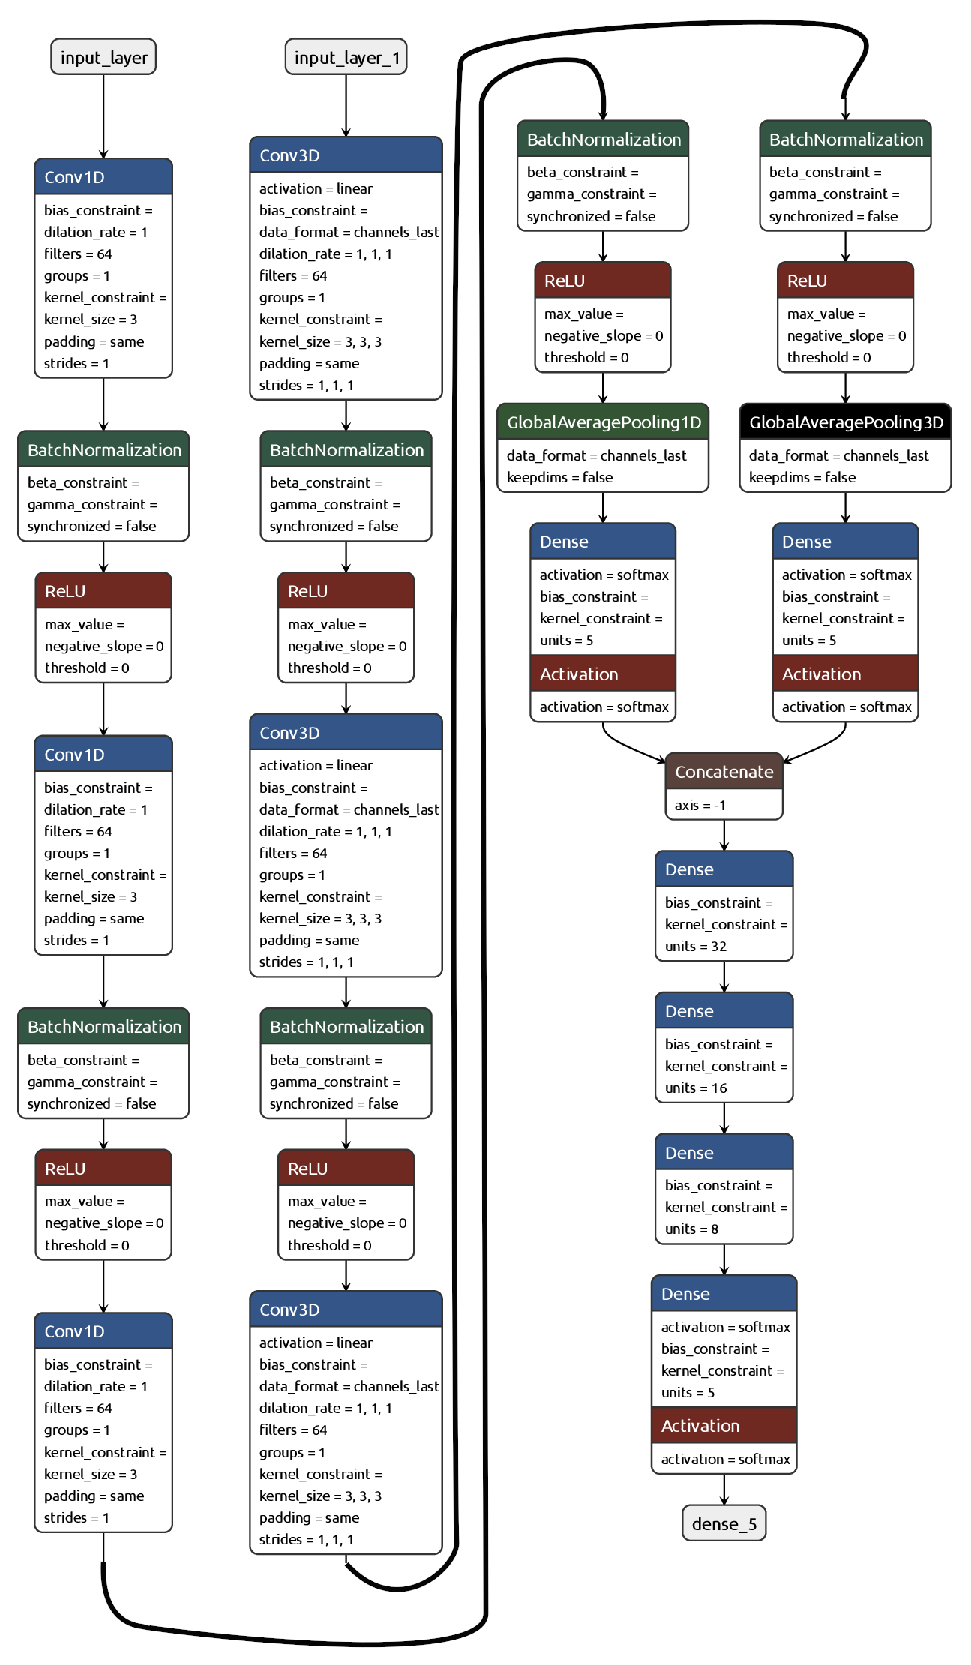
\includegraphics[height=0.7\paperheight]{Figures/3_5_24_model_full.keras}
    \centering
    \caption{Diagram of layers and hyperparameters of the combined motion sickness detection model.}
    \label{fig:model diagram}
\end{figure}
\pagebreak

\subsection{Training}
\label{subsec:training}

The model was compiled using the Adam algorithm for gradient decent and uses categorical cross-entropy as its loss function.
During training, the model was set up to reduce its learning rate (LR) by half when the loss plateaued for 20 epochs to a minimum LR of 0.0001.
It was also set up to end training early if 50 epochs passed with no improvement and would log the loss, accuracy, weights, among other things for each training run.
Lastly, it would save the weights that had created the lowest loss to a file at the end of each epoch.

First, the image and numeric models were trained for 100 epochs maximum to get a clue as to how each separated model performed and to see if they worked properly or needed tweaking.
Every 100 rows of the dataset is a time-period, and is given a rating that is the average of all ratings in the window, and represented as a one-hot vector.
One hundred rows per time-period was chosen as this represents five seconds of application runtime with the application running at 60 frames per second and only every third frame being recorded in the dataset.
The dataset is then split into a training and testing set, where the split is 50\%/50\%.
A split of 80\% training data and 20\% testing data was originally tried, but was found to cause the individual models to overfit and perform poorly in testing.
Time periods were batched together in sets of 2 to make training faster.
Typically, with time series data like this dataset, each time period would be somewhat dependent on the past time-period.
This is still somewhat true, the past time-periods have fairly little impact on the current period.
This means we can shuffle the order of the periods to try and reduce overfitting in the model and help it generalize more effectively.
Only the training data was shuffled.
Lastly, the resolution of the frame images was cut to a fourth as the dataset was loaded to stay within the available system memory of the training machine.
This leaves the images with a result of 256 by 131 pixels.

Training the combined model was much the same as the separated models.
The primary difference is the combine model did not overfit quite as severely and uses the original 80\%/20\% split for training and testing data.
Since the model has two inputs, the numeric data and the image data, both need to be zipped together for each row before being batched into time periods and batches.
Additionally, the combined model was set to train for longer with 250 epochs maximum.

\section{Motion Sickenss Prevention In An Application with Vignetting, Snap Turning, and User Warnings}
\label{sec:prevention}

To apply our model, we created an application that would likely create motion sickness and employed several standard methods for reducing that motion sickness based on the inferences of the model.

\subsection{The Environment}
\label{subsec:environment}

The application was made using the Unity game engine as well as Unity's XR Interaction Toolkit\cite{InteractionToolkit}.
It features two roller-coasters the user can ride, one being a simple circle and the other being more complex.
The user had both continuous and teleport locomotion methods for moving around the environment.
The user enters roller-coasters by pointing at and clicking a button in the environment, after which they will be seated in the roller-coaster's car and will ride along the track.
Afterward, they will be dismounted from the ride and able to walk around again as well as select another coaster to ride.
The environment contains some hills made using Unity's Terrain Generation tools and realistic texturing received from~\url{https://3dtextures.me/}\cite{3dtextures.me}, so the environment resembles those in the dataset instead of a completely flat environment.
The environment is shown in~\ref{fig:environment_images}.
Within this environment, three motion sickness reduction features were implemented.

\begin{figure}[h!]
    \includegraphics[width=\linewidth]{Figures/Environment}
    \centering
    \caption{Two images of the virtual environment from our application: one from the ground(left) and the other on the complex roller coaseter(right)}
    \label{fig:environment_images}
\end{figure}

\subsection{Vignetting}
\label{subsec:vignetting}

Vignetting is the term for reducing the user's FOV with some sort of visual filter akin to a vignette.
This removes visual context suggesting to the user that they are moving, which their vestibular system would contradict, causing motion sickness.
Typically, this is done in games based purely on weather the user is locomoting or not.
In this application, the size of the vignette was determined by the rating provided by the model, where the sicker the user was, the larger the vignette and the less of their periphery the user could see.
The vignetting was provided by Unity's Tunneling Vignette Shader\cite{TunnelingVignette} and examples of our vignetting are shown in~\ref{fig:vignetting_example}.

\begin{figure}[h!]
    \includegraphics[width=\linewidth]{Figures/Vignette}
    \centering
    \caption{The perspective of the user with a black vignette reducing their field of view.}
    \label{fig:vignetting_example}
\end{figure}

\subsection{Snap Turning}
\label{subsec:snap_turn}

Snap Turning refers to larger user rotations that occur instantaneously with a single input.
For instance, the user would press right once on the joystick to ``snap'' 45\textdegree~instantaneously.
This is contrasted by the normal method of holding the joystick right to turn at a constant velocity over time.
This reduces motion sickness by reducing the motion seen but not felt by the user as they rotate over large increments instantly and simply rotate their head for smaller increments.
By default, the application uses continuous turning, unless the user has a motion sickness rating greater than two from the model, where they then use snap rotation at increments of 45\textdegree.

\subsection{User Warnings}
\label{subsec:user_warnings}

Some applications will warn the user to take a break if they have used the application for a certain amount of time.
Our application will display a warning if the model has rated the user as having a motion sickness of five, which is the maximum.
The warning (seen~\ref{fig:user_warning}) tells the user to take a break and is attached to the user's vision.
The warning is removed after five seconds with a lower motion sickness rating from the model.
This is meant as a last resort if nothing can reduce the users' detected sickness as to minimize the effects of prolonged sickness.
Below is an image of said warning.

\begin{figure}[h!]
    \includegraphics[width=\linewidth]{Figures/Warning}
    \centering
    \caption{The perspective of the user with red text near the bottom, stating ``You seem very sick. Please take a break soon!''}
    \label{fig:user_warning}
\end{figure}


\section{Marrying Detection and Prevention}
\label{sec:marrying}

Once the application was built and the model was trained, the two had to be combined.
This was not as easy as one would think.


\subsection{Pulling the necessary data for inference}
\label{subsec: pulling_data}

Pulling controller inputs, and camera matrices were easy as Unity provided functionality to access this data, the device pose was more complicated.
The dataset and therefore the model had recorded the position and rotation of each device in a 4x3 transformation matrix.
Unity, however, provides the position as a vector and the rotation as a quaternion\cite{voight2021quaternion}.
Unity provides a function for retrieving a transformation matrix from a translation(position), rotation, and scale(which would remain as $<1, 1, 1>$).
This function returns a 4x4 matrix, however, where the last row is always $\left[\begin{matrix} 0 & 0 & 0 & 1 \end{matrix}\right]$.
Since the last row is always the same and one row needed to be discarded, the last row was discarded to create the 4x3 matrices needed for the poses.

While originally the numeric and image data from the application would be pulled each frame, this approach introduced massive performance losses.
This is because of how the frame image was represented.
Two images were pulled from the virtual cameras representing the left and right eye's perspective.
They were then attached in one image as a Unity Texture2D\@.
This datatype requires a texture format, and while many are available, none were quite suitable.
The model is trained on IEEE floating point numbers, but most formats were either integers, or compressed formats that would have required decompression.
Of the floating point formats available, the options were RFloat, RGFloat, or RGBAFloat.
The first two formats lack the blue channel the model needs for inference while the last has an additional channel(alpha) that needed to be removed.
To remove the alpha value from the image, we iterated over each value in the image copying it to a float array unless it was the alpha value.
Since iterating over the image, meant iterating over $256*131*4$ or 134144 values, this took considerable time, around 60ms.
However, frames need to be generated in around 18ms and this code would have otherwise held the main thread, reducing the framerate to around 15 frames per second, which would make the user more motion sick among other things.
This required moving the logic into another thread; using Unity's Jobs system.
Jobs maintain thread safety by requiring that the user only work on memory explicitly allocated for the job.
This meant that before starting a job, all data needed for the job would have to be polled, then copied to the job's own memory; then the job could be run.
When the job finished, the data would be copied back from the job's memory back to the main processes' memory.

This culminated in putting together the last one-hundred frames of numeric and image data to be processed in a job.
First, the current time-period would be sent to the job with the new numeric and image data from the current frame.
Jobs also only work with arrays because of specific memory allocation constraints.
Therefore, the job would copy the latest 99 frames from the end of the array containing them to the beginning, and would copy the newest data to the end.
For numeric data, this was simply constituted copying from an array containing that data.
For the new image, each value was iterated through to only copy the red, green, and blue values, but not the alpha values.
Then the job would end and the new data would be copied back.
This process alone would take two or three frames worth of time, meaning the time-period only polled every second or third frame, which matched up with what the model was trained on.
This, however, was only to ready data to be given to the model.

\subsection{Loading the Model in Unity}
\label{subsec:loading}

The model was originally planned to be loaded directly from with Unity.
This would have been possible as Unity uses the C\# programming language, and Microsoft provides a framework for performing ML tasks in their aptly named ML package.
The major benefits of loading the model within C\# are that it's much more performant.
This is because moving data into the model is fast and the ML library can more easily make use of the GPU for influencing than tensorflow from within Windows. % TODO: Cite a source about tf GPU fickleness.
Influencing using the GPU is important as, compared to the CPU, it is much better at handling matrix math and manipulations which primarily make up the computation of CNNs.
Unlike keras, Microsoft's ML package uses a different model storage format and runtime named Onnx.
Converting a keras model to onnx is relatively easy.
However, no matter what was tried, the onnx runtime would not function.

\subsection{Using Inter-Process Communication Instead}
\label{subsec:ipc}

Without the Onnx runtime, we had to use a different method to load the model for influencing.
Since the model would load in python, we decided to load it in python using tensorflow and keras as we did for training.
This necessitated a new process to run the model, separate from the C\# process that gathered the data for inferencing.
This required the use of interprocess communication, specifically sockets.

Sockets are the same thing used to send data over the internet.
Each process creates a socket, one process is a server waiting for clients to connect, clients then connect and send data, the server sends data back.
In this case, the python process with the model would be the server and would have to take care to manage the connection received by the C\# process.
The python server would wait for a connection, receive the data it needed for inference, get a rating for the user's motion sickness, and send that rating back to the client, and finally disconnect.

One would think to hold open the connection and let both processes talk until either ended.
However, because getting GPU inferencing to work in Windows within TensorFlow is rather finicky, CPU inferencing, which is much slower, is needed instead.
This slowness, like with the image iterations, would have wreaked havok on performance, so the C\# process needed to communicate with the python process through a job on a separate thread.
Since jobs have their own segment of memory that cannot be shared with the main process, the connection cant be passed between the main thread and the job.
The job also can't hold onto the connection as its memory is deallocated when the job is complete, unless it's copied back to the main process, which couldn't be done.
This necessitated creating a new socket connection to the python server for every job (which occurs every 2 to 15 frames), after the processing of the new frame's data was completed.
Once the inference was received, the job would terminate and the prediction would be passed back to the main thread to be handed to the C\# that handled the motion sickness mitigations.

\chapter{RESULTS}
\label{ch:results}

The model was quite accurate on the testing portion of the dataset.
The separate numeric and image models each attained about 60\% accuracy.
This isn't great but much better what would be 20\% if the model were guessing randomly.
The combined model, however, got an accuracy score of 85\%.
This is significantly better than either of the separate models.
However, the model's accuracy on the dataset is not the same as its real-world efficacy.
Most rows in the dataset are rated as a one of five, meaning a decent accuracy can be achieved by simply assuming 1 if no better rating can apply.

The model's predictions apply decently well to a real-world application.
When the user looking around or physically walking around, the model rates them as having no motion sickness (rating of 1).
This means the model is not rating the user as sick when the user is moving in a way that does not confuse their vestibular system.
In contrast, the model rates them as being slightly sick (rating of 2) when the user moves using their joystick.
This is good as the model is not overreacting and can differentiate between motion that the user can physically feel and motion that is only seen.
Not only that, but this behavior effectively re-implements locomotion-based vignetting, which is common in most VR applications.
When the user is riding a rollercoaster and looking forward, the user is rated as moderately sick (rating of 3).
This rating being higher than walking is expected, but the model does not overreact and apply the highest rating which is good.
When the user isn't looking forward to the rollercoaster but to the side, the model rates the user as either not sick or low sickness (rating 1--2).
This makes sense as the user is perceiving motion for objects in the environment where looking forward the motion could only be perceived as the user's movement.
The model also detects when the user removes their headset, stating there is no motion sickness (rating of 1).
This is interesting as the model receives no specific data the headset was removed.
As well, the model is not detected when the headset is set down, and its velocity is zero but specifically when the headset is removed.
These results are all tabulated in~\ref{tab:predictions}

\begin{table}[h!]
    \centering
    \begin{tabular}{|l|l|l|}
        \hline
        Stimuli                                & Predicted Sickness Rating & Mitigations Applied  \\ \hline
        Looking~(Physical)                      & 1                         & None                 \\ \hline
        Looking~(Locomotion)                    & 1                         & None                 \\ \hline
        Teleportation                          & 1                         & None                 \\ \hline
        Walking~(Physical)                      & 1                         & None                 \\ \hline
        Walking~(Locomotion)                    & 2                         & Vignetting(Light)    \\ \hline
        Simple Roller Coaster                  & 3                         & Vignetting(Moderate) \\ \hline
        Complex Roller Coaster~(Facing Forward) & 3                         & Vignetting(Moderate) \\ \hline
        Complex Roller Coaster~(Facing to Side) & 1                         & None                 \\ \hline
        Headset Removed                        & 1                         & None                 \\ \hline
    \end{tabular}
    \caption{Infrences by the motion predition model on various stimuli. Stimuli marked ``Physical'' refer to the user physically moving where stimuli marked ``Locomotion'' refer to the user acting with the controllers.}
    \label{tab:predictions}
\end{table}

The performance overhead of this system is significant.
With the model and data formatting operations, the application takes 30 to 40ms to produce a frame compared to 16ms without them.
This equates to a frame rate of 30 frames per second.
This is not unusable but may cause more motion sickness, and for performance critical applications this may just not be feasible to apply.
This performance is in part due to bad implementation.
Assuming the model was inferencing using the GPU and a better method of loading and passing data to the model were found, and less image processing had to be done, the overhead could be significantly reduced.
These could easily be resolved with more time.

\chapter{CONCLUSION}
\label{ch:conclusion}

In conclusion, using a CNN to manage motion sickness mitigation in a VR application is absolutely feasible given that the overhead from the model is taken into account.
We used the VRNet motion sickness dataset and created an ensemble model that could predict with an accuracy of 85\% on the held-out samples of the dataset.
We created an example VR application with a somewhat detailed environment and motion sickness mitigations.
When the model was put in control of those mitigations, it made decisions that were fairly logical, though with some performance concerns.

\section{Future work}
\label{sec:future_work}
The obvious first steps are to make influencing and collection of data from the engine more efficient.
Beyond this, the model could be extended to increase accuracy by adding ``Long Short-Term Memory'' (LSTM) layers so the model can make more improved predictions.
Note that this would require not shuffling the trained time periods.
There are other motion sickness mitigation features that could be implemented and controlled by the model.
A dataset that could classify the user's motion sickness by cause could provide more specific mitigations by reducing the specific cause of motion sickness.
A better model and more performant application should be tested on real users to see its real world efficacy.
If all these things were done and the improved application was proven to cause less motion sickness, this system could be deployed in many applications to reduce motion sickness at the best time, before it happens.



%Intro
%  Problem Statement
%  Objectives
%  Literature Review
%Methods
%  Motion Sickenss Detection with Convolutional Neural Networks
%    Dataset
%	Network Achitecture
%	Training
%  Motion Sickenss Prevention with Vignetting, Snap Turning, and User Warnings
%    Vignetting
%	Snap Turning
%	User Warnings
%  Marrying Detection and Prevention
%    Loading the Model in Unity
%	Using Inter-Process Communication Instead
%Results
%  Model Predictions
%  Model Accuracy
%  Application Performance
%Conclusions
%  Future Work
%Appendex
%Bibliograpy




% 
% The bibliography page must be between main body and appendices
%
% You must have thbib.bib file in the current directory 
%
% (uncomment \nocite{*} to force inclusion of all uncited entries)
% \nocite{*}
\bibliographystyle{IEEEtran}
\bibliography{bibi}

% This includes append.tex
%\appendices
%
% If you only have one appendix, you should change the above to:
%\appendix
%

\chapter{MORE INFORMATION ON EQUATIONS}

To demonstrate how an appendix should be inserted into the thesis we
have provided two appendices. This first appendix illustrates some
more advanced techniques to improve the appearance of your equations.
Below is a system of partial differential equations from a model for
cellular control by an external nutrient. The equations are
complicated and \LaTeX\ tends to allow them to run into each other. To
prevent this we have used the \verb+\vrule+ command to separate
them. Note this is an ordinary \TeX\ command and is not in L.\
Lamport's book \cite{LAM}. Furthermore, we have some complicated
boundary conditions that we needed to align, so we used the array
command, but to get the equations looking right we also needed the
\verb+\dfrac+ command instead of the \verb+\frac+ command. The
equations for our model are as follows:
\begin{eqnarray}
  \dot{U}_1(t) & = & \tilde f(W_1(t-T)) - U_1(t) + \gamma_1U_2(R\sigma,
   t){\vrule width 0in depth .1in},	\nonumber \\
  \dot{W}_1(t) & = & -\hat b_3W_1(t) + \gamma_3W_2(R\sigma,
   t){\vrule width 0in depth .1in},\nonumber \\
  \frac{\partial U_2}{\partial t} & = & D_1\nabla^2U_2 - U_2 - \tilde f(W_1
    (t-T)) - \gamma_1U_2(R\sigma,t){\vrule width 0in depth .1in},
	\label{sys2} \\
  \frac{\partial V_2}{\partial t} & = & D_2\nabla^2V_2 - b_2V_2 + c_0
    \bigl(U_2 + U_1(t)\bigr){\vrule width 0in depth .1in}, \nonumber \\
  \frac{\partial W_2}{\partial t} & = & D_3\nabla^2W_2 - b_3W_2 + (\hat b_3
    -b_3)W_1 - \gamma_3W_2(R\sigma,t) \nonumber \\
    &  & + k\left[\left[{\left(\frac{D_3}{r^2}\right)}\frac{d}{dr}\left(r^2
	   \frac{dh}{dr}\right) - b_3h\right]V_2(R,t) - h\dot V_2(R,t)
	   \right], \nonumber
\end{eqnarray}
for $t > 0$ and $R\sigma < r < R$ and with the boundary conditions:
\begin{equation*}
\begin{array}{rclcrcl}
 \dfrac{\partial U_2(R\sigma,t)}{\partial r} & = &
   \beta_1U_2(R\sigma,t), & \qquad &
 \dfrac{\partial U_2(R,t)}{\partial r} & = &
   0, \\
\\
 \dfrac{\partial V_2(R\sigma,t)}{\partial r} & = &
   0, & \qquad &
 \dfrac{\partial V_2(R,t)}{\partial r} & = &
   0, \\
\\
 \dfrac{\partial W_2(R\sigma,t)}{\partial r} & = &
   \beta_3W_2(R\sigma,t), & \qquad &
 \dfrac{\partial W_2(R,t)}{\partial r} & = &
   0.
\end{array}
\end{equation*}
Notice that the system is numbered only once by (\ref{sys2}) and that
this is centered as best we can on one line. All other lines have the
$\backslash$\textit{nonumber} command.


\chapter{LISTS AND QUOTATIONS}

The thesis will rarely use list environments, but they are valuable
for r{\'e}sum{\'e}s. For more information on creating a r{\'e}sum{\'e}
you may want to see the author of this document (you also need to
learn quite a bit about \verb+\parbox+ commands).  To create a list
you will want to use one of \texttt{itemize, enumerate,} or
\texttt{description}. For example:
\begin{description}
\item[continuous] A function $f$ is {\bf continuous} at $x$ if and only
if for every $\varepsilon >0$ there exists a $\delta(x) >0$ such that
whenever $|y-x|<\delta$, $|f(y)-f(x)| < \varepsilon$.
\item[uniformily continuous] A function $f$ is {\bf uniformly
continuous} if and only if for every $\varepsilon >0$ there exists a
$\delta >0$ such that whenever $|y-x|<\delta$, $|f(y)-f(x)| <
\varepsilon$ independent of $x$ and $y$.
\item[equicontinuous] A family of functions $f_n$ is {\bf
equicontinuous} at a point $x$ if and only if for every $\varepsilon >0$
there exists a $\delta >0$ such that whenever $|y-x|<\delta$,
$|f_n(y)-f_n(x)| < \varepsilon$ for all functions $f_n$.
\end{description}

\LaTeX\ provides an environment for block quotations. To agree with standard 
thesis formatting manual follow the format below for a quotation exceeding four
lines. From Lewis Carrol's {\it Hunting of the Snark} we hear the
Bellman tell his crew:
 \vspace{.12pt}

{
\ssp
\begin{verse}
The Bellman himself they all praised to the skies--\\
Such a carriage, such ease and such grace!\\
Such solemnity, too! One could see he was wise,\\
The moment one looked in his face!\\
 \vspace{.15in}
He had bought a large map representing the sea,\\
Without the least vestige of land:\\
And the crew were much pleased when they found it to be\\
A map they could all understand.\\
 \vspace{.15in}
``What's the good of Mercator's, North Poles and Equators,\\
Tropics, Zones, and Meridian Lines?''\\
So the Bellman would cry: and the crew would reply,\\
``They are merely conventional signs!''\\
 \vspace{.15in}
``Other maps are such shapes, with their islands and capes!\\
But we've got our brave Captain to thank''\\
(So the crew would protest) ``that he's bought us the best--\\
A perfect and absolute blank!''\\
\end{verse}
}




\end{document}
